%% intro.tex
%%
%% Copyright 2017 Evandro Coan
%% Copyright 2012-2016 by abnTeX2 group at http://www.abntex.net.br/
%%
%% This work may be distributed and/or modified under the
%% conditions of the LaTeX Project Public License, either version 1.3
%% of this license or (at your option) any later version.
%% The latest version of this license is in
%%   http://www.latex-project.org/lppl.txt
%% and version 1.3 or later is part of all distributions of LaTeX
%% version 2005/12/01 or later.
%%
%% This work has the LPPL maintenance status `maintained'.
%% The Current Maintainer of this work is the Evandro Coan.
%%
%% The last Maintainer of this work was the abnTeX2 team, led
%% by Lauro César Araujo. Further information are available on
%% https://www.abntex.net.br/
%%
%% This work consists of a bunch of files. But originally there ware 3 files
%% which are renamed as follows:
%% Renamed the `abntex2-modelo-include-comandos` to `chapters/chapter_1.tex`
%% Renamed the `abntex2-modelo-trabalho-academico.tex` to `chapters/intro.tex`
%% Renamed the `abntex2-modelo-references.bib` to `aftertext/modelo-ufsc-references.bib`
%%
%% This file was originally the main template file, however this main file was
%% split into several new files, which are respectively drastically changed,
%% except this files which contains most of the main documentation message.
%%

% ------------------------------------------------------------------------
% ------------------------------------------------------------------------
% abnTeX2: Modelo de Trabalho Academico (tese de doutorado, dissertacao de
% mestrado e trabalhos monograficos em geral) em conformidade com
% ABNT NBR 14724:2011: Informacao e documentacao - Trabalhos academicos -
% Apresentacao
% ------------------------------------------------------------------------
% ------------------------------------------------------------------------

% The \phantomsection command is needed to create a link to a place in the document that is not a
% figure, equation, table, section, subsection, chapter, etc.
% https://tex.stackexchange.com/questions/44088/when-do-i-need-to-invoke-phantomsection
\phantomsection

% https://tex.stackexchange.com/questions/5076/is-it-possible-to-keep-my-translation-together-with-original-text
\chapter{\lang{Introduction}{Introdução}}\label{chap:intro}
\phantomsection

In the realm of mathematical optimization, Mixed-Integer Linear Programming (MILP) stands as a powerful tool for addressing a wide array of complex decision-making problems.
These problems, prevalent in fields ranging from operations research to finance and logistics, often involve the need to make discrete decisions within a linear framework.
Despite their significance, solving MILP instances efficiently remains a formidable challenge, as the search space expands exponentially with the number of integer variables.
In other words, the combinatorial nature of MILP implies that algorithms with optimality guarantees have intractable running times.

Primal heuristics, which aim to quickly finding high-quality feasible solutions to MILP problems, play a crucial role in enhancing the efficiency of optimization algorithms.
Traditional primal heuristics are often rule-based and designed to exploit structures of a given MILP problem.
As a consequence, they lack adaptability, struggling to generalize across diverse problem instances.
As the landscape of optimization problems continues to evolve, there is a growing need for intelligent and flexible heuristics that can adapt to the intricacies of different MILP instances.

% TODO: add references to "successfully applied to MILP"
Recently, deep learning techniques have been successfully applied to MILP, resulting in effective heuristics.
In contrast to handcrafted heuristics, which rely on expert knowledge to exploit theoretical structures of problem formulations, deep learning-based heuristics identify the hidden patterns of problem instances from data.
This data-driven approach relies on the assumption that problem instances are drawn from underlying distributions, and, thus, share characteristics not evident in the mathematical formulation.
Such assumption often holds for practical situations, in which problems must be solved repeatedly and the parameters that define the instances are random variables with unknown distributions.

The research area of deep learning applications to MILP has seen a burst in publications in the past years, as can be seen in Fig. \ref{fig:scopus-trend}, with plenty of novel methods being proposed.
The comparisons, however, are still limited, which hinders the effective application of the approaches available in the literature.
In this context, this master's thesis aims to contribute to the development of learning-based heuristics for MILP problems by evaluating existing techniques in novel applications.
More specifically, this work focuses on deep learning models trained with supervision to predict solutions to MILP problems.

\begin{figure}[h]
    \centering
    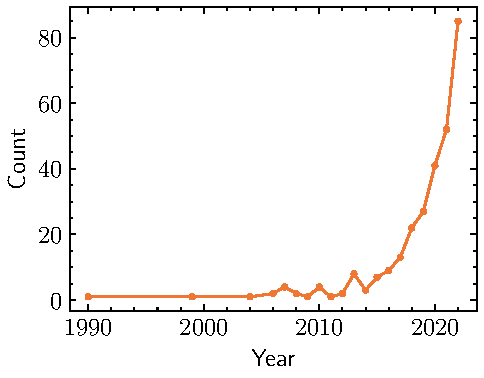
\includegraphics[width=0.8\textwidth]{pictures/scopus.pdf}
    \caption{Number of scientific publications (journal and conference papers) in English language containing the terms "learning" and "MILP" in their title, abstract or keywords. Source: SCOPUS}
    \label{fig:scopus-trend}
\end{figure}

\section{Objectives}\label{chap:objectives}

In the topic of this thesis, three research questions are of fundamental importance in the development of heuristic approaches:
\begin{itemize}
    \item How to design deep learning models able to provide candidate solutions for instances of an MILP problem?
    \item Which supervised learning techniques are most effective to train solution prediction models for primal heuristics? And
    \item How to incorporate solution prediction models in primal heuristics?
\end{itemize}
Targeting these questions, the main goal of this thesis is \emph{to evaluate primal heuristics for MILP problems based on solution prediction models trained with supervised learning techniques}.
This goal is broken down into two objectives:
\begin{itemize}
    \item To assess the literature on supervised learning solution prediction models for MILP problems, including model architectures, supervised learning algorithms, and learning-based primal heuristics; and
    \item To evaluate the most promising techniques in a realistic application with respect to the performance of the resulting primal heuristic.
\end{itemize}
It is expected that the successful achievement of these objectives will result in the two major contributions of this work to the research community.

